\subsection{Elektromagnet-kraftmåling}\label{bilag_elektromagnet}
\label{Elektrojournal}
\subsubsection*{Formål}
Formålet med denne journal er at undersøge effektiviteten af en elektromagnet. Elektromagneten skal bruges til at holde bilen på banen i sving. Resultatet af denne journal vil bruges i bedømmelsen om hvorvidt en elektromagnet er hensigtsmæssigt på bilen. Der laves en prøve magnet, der har pasform til at kunne placeres under bilen. Samtidig skal der testes for hvor meget kraften falder, i forhold til afstand mellem magneten og banen. Derudover testes den permanente magnet for hvor kraftig den er og sammenlignes herefter med elektromagneten.\\
\\
\subsubsection*{Materiale liste}
\begin{itemize}
	\item Materiale af stål
	\item Kobbertråd af 0.25 mm
	\item Strømforsyning
	\item Pasco Force sensor
	\item Bilens permanent magnet
	\item Magnetisk metal plade
	\item Papir af 0.2 mm tykkelse
	\item Program, PASCO capstone
	\item Computer
\end{itemize}
 
\subsubsection*{Opstilling}

\begin{figure}[h!]
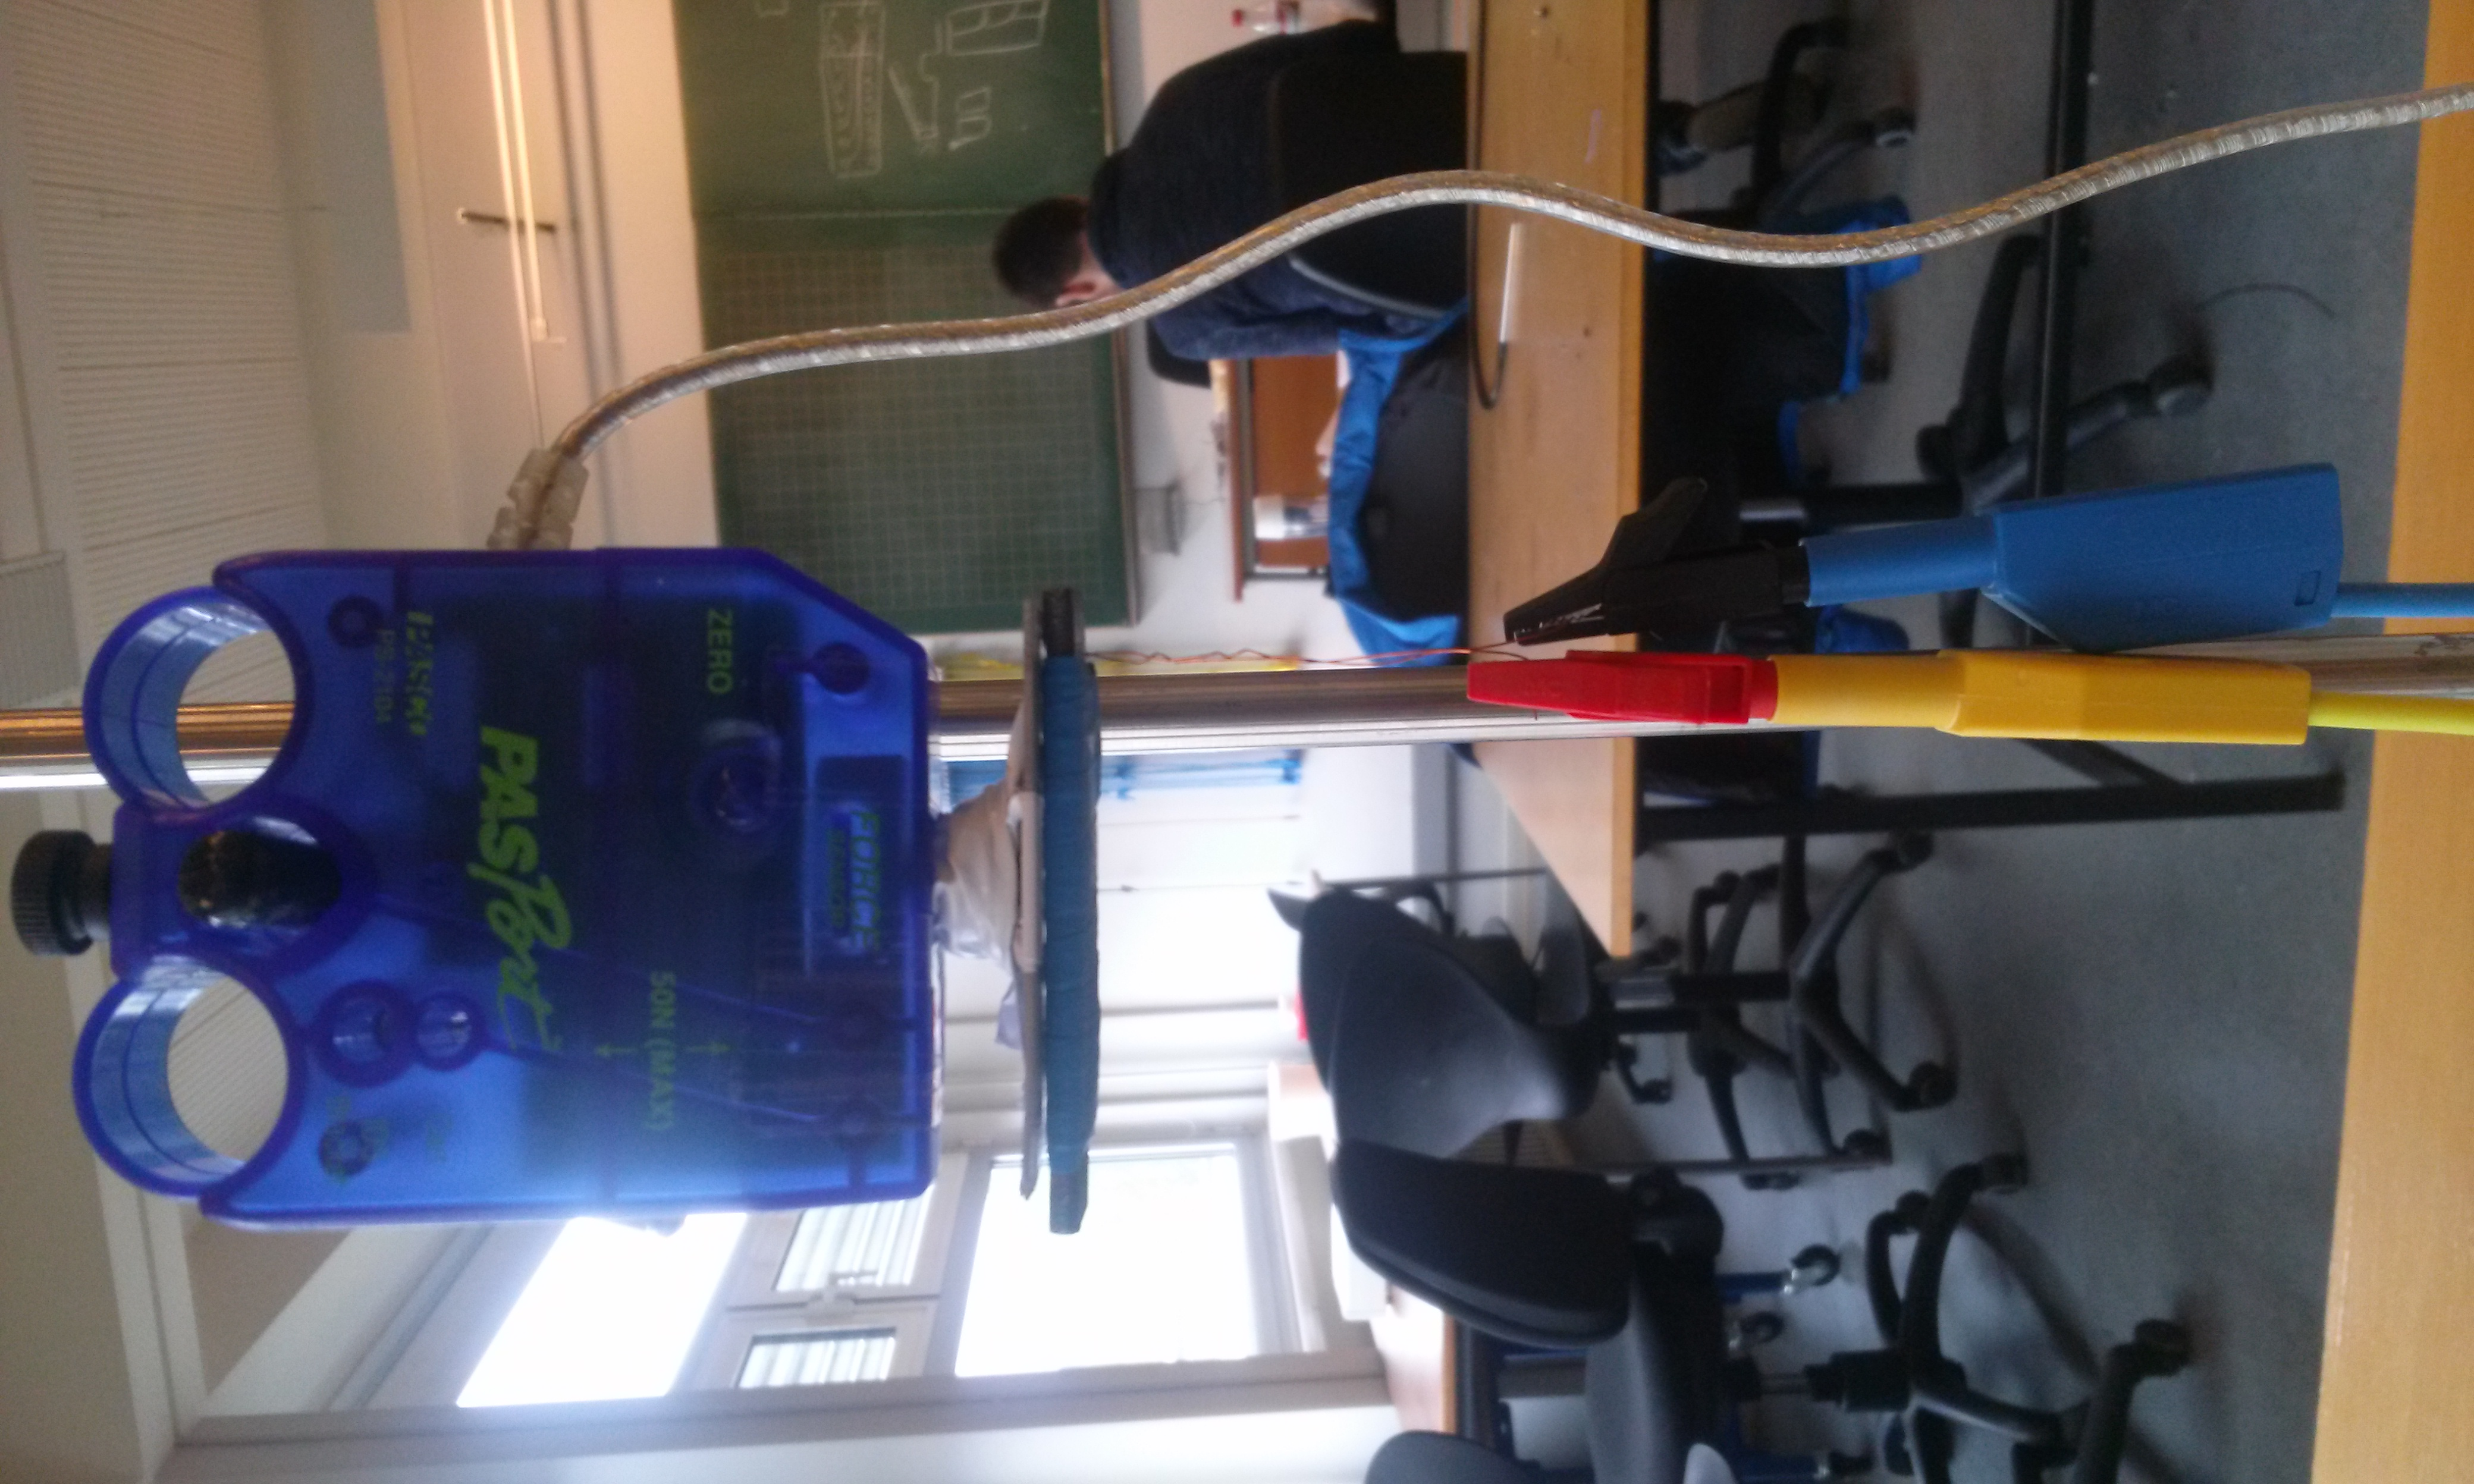
\includegraphics[scale=0.04, angle=270]{./Graphics/Forsogs_opstilling}
\caption{Forsøgsopstilling for elektromagnet på kraftsensor}
\label{Opstilling}
\end{figure}

\begin{enumerate}
	\item Der skæres og slibes en magnet af ferromagnetisk materiale. 
	\item Der vikles vindinger rundt om magneten indtil en bredde på ca. 4mm er opnået. Der er 6mm fra bilens undervogn til banen, derfor skal der måles med en afstand på 2mm luftgab.
	\item Force sensoren placeres så den kan måle magnetens kraft, når den trækkes af en metalplade. 
	\item En computer med programmet PASCO capstone bruges til at læse kraftmålingerne.\\
 \end{enumerate}
  
Forsøget går ud på at lave en elektromagnet der kan sidde under bilen, derfor laves en test magnet med 660 vindinger, da der ikke kan være flere vindinger. En kraftmåler opstilles så den måler begge elektromagnetens ender, der sættes 14V og 1,4A over elektromagneten og kraften måles nu ved at trække elektromagneten af kraftmåleren. Forsøget gentages nu, med et stykke papir på 0.2mm, dernæst 0,4mm, indtil vi når op på 2mm. Forsøget gentages med Permanentmagneten og målingerne gemmes på computer. \\



\subsubsection*{Data}
Data i figur \ref{elektrotabel} er et førsøg der er gentaget 3 gange og og luftgabet er lavet med flere stykker 0.2 mm papir, resultaterne er i Newton. \\
\begin{figure}[h!]
\begin{tabular}{|c|c|c|c|c|c|c|c|c|c|c|c|}
\hline 
Luftgab & 0 & 0.2 & 0.4 & 0.6 & 0.8 & 1 & 1.2 & 1.4 & 1.6 & 1.8 & 2 \\ 
\hline 
Forsøg 1 & 1.345 & 1.320 & 1.090 & 1.100 & 1.090 & 1.130 & 1.060 & 1.090 & 0.930 & 0.970 & 0.960 \\ 
\hline 
Forsøg 2 & 1.570 & 1.150 & 1.350 & 1.320 & 1.120 & 1.050 & 1.000 & 1.060 & 1.040 & 0.950 & 0.870 \\ 
\hline 
Forsøg 3 & 1.000 & 1.440 & 1.350 & 1.100 & 1.200 & 1.200 & 1.200 & 1.100 & 1.000 & 0.930 & 0.980 \\ 
\hline 
Gennemsnit & 1.305 & 1.303 & 1.263 & 1.173 & 1.137 & 1.127 & 1.087 & 1.083 & 0.990 & 0.950 & 0.937 \\ 
\hline 
\end{tabular}
\caption{Elektromagneten}
\label{elektrotabel}
\end{figure} \\

Data i figur \ref{permtabel} er fra målinger af permanetmagneten.\\

\begin{figure}[h!]
\begin{tabular}{|c|c|c|c|c|c|c|c|c|c|c|c|}
\hline
Luftgab & 0 & 0.2 & 0.4 & 0.6 & 0.8 & 1.0 & 1.2 & 1.4 & 1.6 & 1.8 & 2 \\
\hline
Forsøg 1 & 4.20 & 4.82 & 3.34 & 4.17 & 4.12 & 4.14 & 3.25 & 2.97 & 2.18 & 2.52 & 1.65 \\
\hline
Forsøg 2 & 4.38 & 4.65 & 4.74 & 4.90 & 4.40 & 4.23 & 3.41 & 2.38 & 2.30 & 2.18 & 1.31 \\
\hline
Forsøg 3 & 4.67 & 4.95 & 4.37 & 4.79 & 4.12 & 3.44 & 3.30 & 1.96 & 1.85 & 1.65 & 1.48 \\
\hline 
Gennemsnit & 4.42 & 4.81 & 4.15 & 4.62 & 4.21 & 3.94 & 3.32 & 2.44 & 2.11 & 2.12 & 1.48 \\
\hline
\end{tabular} 
\caption{Permanentmagneten}
\label{permtabel}
\end{figure}

\subsubsection*{Resultater}
\begin{figure}[h!]
\center
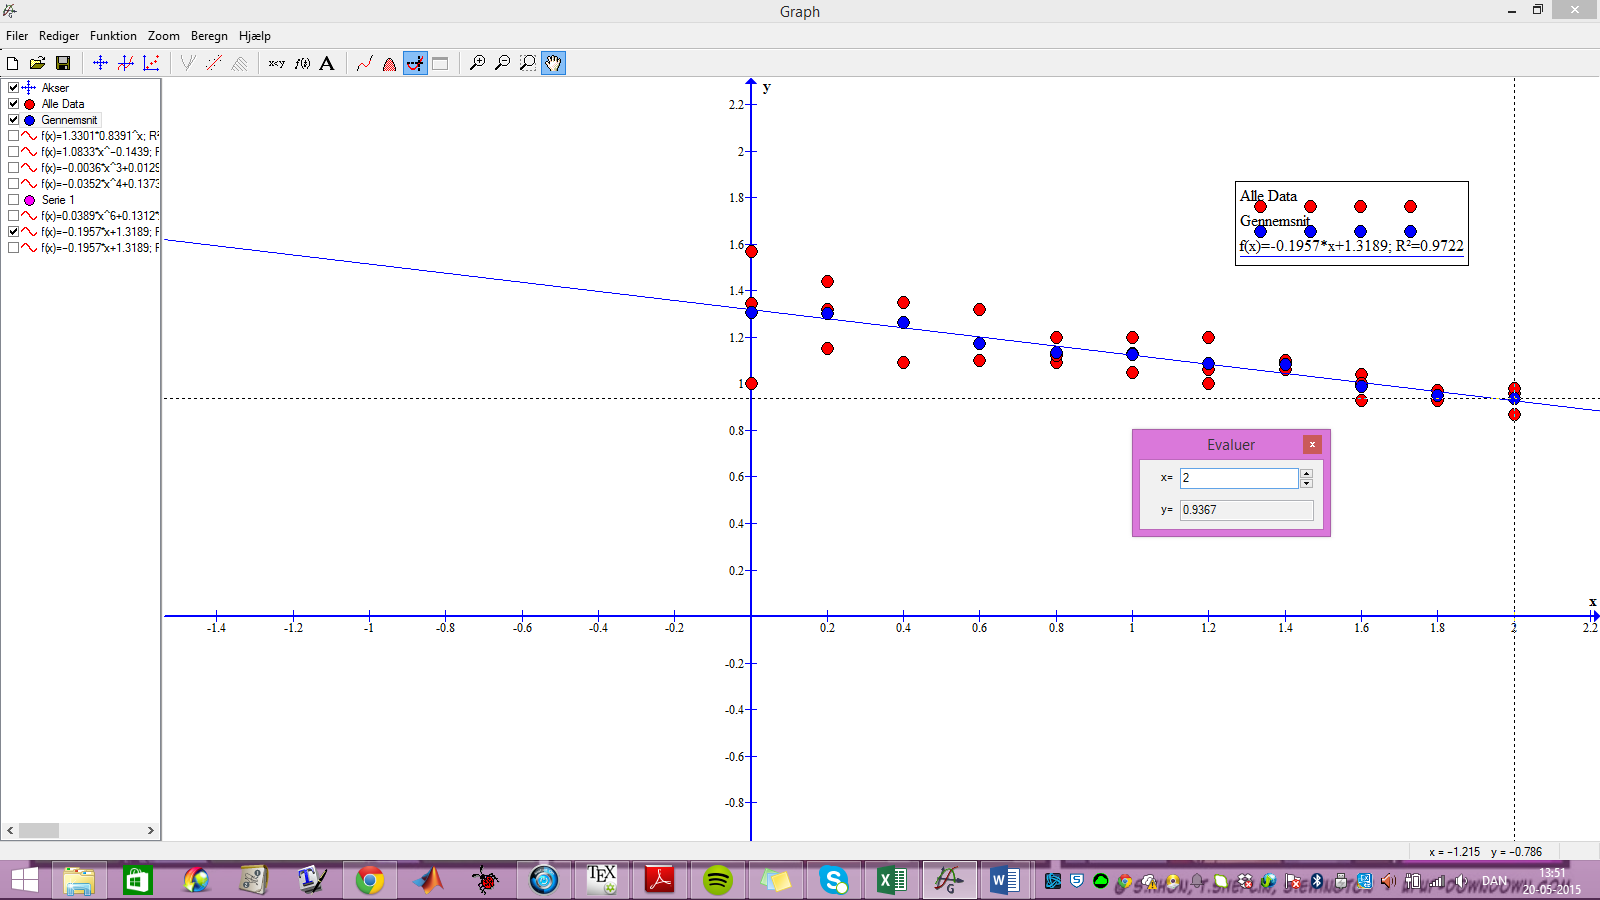
\includegraphics[scale=0.3]{./Graphics/Graf_Elektromagnet_resultater}
\caption{Data sættet for elektromagnet behandlet i graf}
\label{Elektromagnet}
\end{figure}

Her ligger punkterne over datasættet, hvor de røde punkter er data for alle forsøgene og de blå er gennemsnittet af disse forsøg. Vi får nu at der er en kraft på 0.9367 N, ved luftgabet på 2 mm.

\subsubsection*{Udregninger}
Vi udregner hvordan elektromagneten ville virke under ideele forhold, det vil sige hvis, der ikke var nogen fluxspredning i elektromagneten. For udregningerne antages det at materialet er en legering af jern, som ligger mellem 300-500 relativ permeabilitet.\\

$H_{j}l_{j}+2H_{g}x=IN$ \\

$H_{j}=\frac{B_{j}}{\mu_{0}\mu_{r}},\,H_{g}=\frac{B_{g}
}{\mu_{0}}$\\

Ved at antage at der ikke er nogen spredning i luftgabet er $B_{g}=B_{j}$ som nu giver:\\

$\frac{B_{g}}{\mu_{0}\mu_{r}}*l_{j}+2*\frac{B_{g}}{\mu_{0}}=IN$\\

$B_{g}$ isoleres og nu har vi ligningen:\\

$B_{g}(x)=\frac{\mu_{0}IN}{({\frac{l_{j}}{\mu_{r}}}+2x)}$\\

Da elektromagneten er en jern legering vil permeabiliteten ligge mellem 300-500, derfor regnes $B_{g}$ nedre og øvre grænse.\\

$B_{g,Min}(x)=\frac{1,256*10^{-6}*1,4A*660}{\frac{0,07m}{300}+2*0,002m}=0,27 T$\\

$B_{g,Max}(x)=\frac{1,256*10^{-6}*1,4A*660}{\frac{0,07m}{500}+2*0,002m}=0,28 T$\\

Her kan vi se at forskellen i permeabiliteten ikke har den store betydning når det kommer til udregning af magnetisk induktion (B) og Magnetisk feltstyrke (H). 
De næste beregninger gælder for luftgab:\\

$U_{B}=\frac{1}{2\mu_{0}}*\frac{(\mu_{0}IN)^{2}}{({\frac{l_{j}}{\mu_{r}}}+2x)^{2}}*A_{j}*x$ \\

Den magnetiske kraft kan findes ud fra $F_{magn,x}=\frac{dU_{B}}{dx}$ \\
Hvilket giver:\\
$F_{magn,x}=A_{j}*\frac{(\mu_{0}IN)^{2}}{2\mu_{0}}*\frac{1}{(\frac{l_{j}}{\mu_{r}}+2x)^{2}}+x*(-2)*\frac{2}{(\frac{l_{j}}{\mu_{r}}+2x)^{3}}$\\

Eller ved at reducere udtrykket:\\
$F_{magn}(x)=-{\frac{B^{2}_{g}}{2\mu_{0}}}* {A_{j}}* (\frac{4x}{{\frac{l_{j}}{\mu_{r}}}+2x}-1) $\\

Nu kan kraften ideelt set regnes ud:\\
$ F_{magn,Min}=-\frac{0,27T^{2}}{2*1,256*10^-6}*4,5m^2*10^{-5}*(\frac{4*0,002m}{\frac{0,07m}{300}+2*0,002m}-1)=-1,1619N $\\

$ F_{magn,Min}=-\frac{0,28T^{2}}{2*1,256*10^-6}*4,5m^2*10^{-5}*(\frac{4*0,002m}{\frac{0,07m}{500}+2*0,002m}-1)=-1,309N $\\

Minustegnet indikerer at kraften virker nedad i samme retning som tyngdekraften.\\

\subsubsection*{Konklusion}
Ud fra data og beregninger kan man hurtigt konkludere at elektromagneten ikke er ideel, da der er et tab på $0,2249-0,372$N ved en afstand på 0,2 mm fra skinnerne. Tabet er blandt andet fluxspredning og fluxfringing. Derudover kan man se på dataerne fra permanentmagneten at de falder og stiger hurtigt og er meget varierende, men som udgangspunkt går vi ud fra at de er rigtige. Permanentmagneten er 0,543N stærkere end elektromagneten ved de 0,2 mm afstand fra banen.  


